%%%%%%%%%%%%%%%%%%%%%%%%%%%%%%%%%%%%%%%%%
% University/School Laboratory Report
% LaTeX Template
% Version 3.1 (25/3/14)
%
% This template has been downloaded from:
% http://www.LaTeXTemplates.com
%
% Original author:
% Linux and Unix Users Group at Virginia Tech Wiki
% (https://vtluug.org/wiki/Example_LaTeX_chem_lab_report)
%
% License:
% CC BY-NC-SA 3.0 (http://creativecommons.org/licenses/by-nc-sa/3.0/)
%
%%%%%%%%%%%%%%%%%%%%%%%%%%%%%%%%%%%%%%%%%

%----------------------------------------------------------------------------------------
%	PACKAGES AND DOCUMENT CONFIGURATIONS
%----------------------------------------------------------------------------------------

\documentclass{article}
\usepackage[utf8]{inputenc}
\usepackage{appendix}
\usepackage[T1]{fontenc}
\usepackage{siunitx} % Provides the \SI{}{} and \si{} command for typesetting SI units
\usepackage{graphicx} % Required for the inclusion of images
\usepackage{natbib} % Required to change bibliography style to APA
\usepackage{amsmath} % Required for some math elements
\usepackage{caption}
\usepackage{tikz}


\usepackage{float}


\usetikzlibrary{arrows,automata, positioning}

\usepackage{import}

\setlength\parindent{0pt} % Removes all indentation from paragraphs

%----------------------------------------------------------------------------------------
%	DOCUMENT INFORMATION
%----------------------------------------------------------------------------------------

\title{Prova Finale di Reti Logiche} % Title
\author{Montanari Tommaso e Negri Riccardo} % Author name
\date{1 Aprile 2022}

\begin{document}
\maketitle % Insert the title, author and date
\begin{center}
\begin{tabular}{l l l l}
Docente: & Salice Fabio & & \\ 
Studente 1: & Montanari Tommaso & 10661941 & 932673\\
Studente 2: & Negri Riccardo & 10729927 & 936820 
\end{tabular}
\end{center}

% If you wish to include an abstract, uncomment the lines below
% \begin{abstract}
% Abstract text
% \end{abstract}

%----------------------------------------------------------------------------------------
%	SECTION 1
%----------------------------------------------------------------------------------------

\section{Introduzione}

La prova prevede l'implementazione in VHDL di una macchine che opera su una memoria e svolge la seguente operazione.

La macchina deve per prima cosa leggere il primo byte dalla memoria che identifica il numero di parole che sono
state fornite come input, questa informazione è importante per capire quando la macchina deve terminare la lettura.

Dopodiché ogni parola successiva viene tradotta in due parole di memoria che vengono scritte progressivamente in un'altra parte della memoria.

Le parole di memoria sono interpretate com un flusso continuo e l'uscita è un flusso di lunghezza doppia. Visto che i byte vengono tradotti come un unico flusso l'output di una certa parola dipende anche da quelle precedenti e non possono essere processate separatamente.

\subsection{Esempio}

\begin{tabular}{c c c}
	Indirizzo & Valore & Codifica binaria \\
	0 & 2 & 0000 0010 \\
	1 & 35 & 0010 0011 \\
	2 & 161 & 1010 0001 \\
\end{tabular}
\\
\\
Questo stato della memoria si traduce nell'input [35, 161] e in questo caso la lunghezza dell'input W=2 quindi mi aspetto una lunghezza dell'output Z=4.
\\
\\
\begin{tabular}{c c c}
	Indirizzo & Valore & Codifica binaria \\
	1000 & 13 & 0000 1101 \\
	1001 & 206 & 1100 1110 \\
	1002 & 97 & 0110 0001 \\
	1003 & 195 & 1100 0011 \\
\end{tabular}
\\
\\
Rappresenta l'output [13, 206, 97, 195] dove la codifica dei numeri [13, 206] è l'output prodotto dai bit dal 35 in ingresso. Mentre [97, 195] sono il risultato dei bit presenti nella la codifica di 161.

\subsection{Ipotesi Progettuali}
\begin{itemize}
\item {Si utilizza la scheda Artix-7 FPGA xc7a200tfbg484-1}
\item {Ogni byte può contenere numeri da 0 a 255.}
\item {La quantità di numeri in ingresso (W) è contenuta in una parola da un byte quindi anche il numero massimo di parole da tradurre è 255.}
\item {Dato che l'input occupa al massimo 256 byte posso scrivere sui byte successivi quindi l'output parte sempre dal millesimo indirizzo di memoria che sicuramente non contiene l'input}
\end{itemize}

\subsection{Segnali}
\begin{itemize}
	\item \textbf{i\_clk:} Segnale di clock
	\item \textbf{i\_rst:} Segnale di reset, deve riportare la macchina allo stato iniziale.
	\item \textbf{i\_start:} Quando viene portato a 1 la macchina comincia ad operare e prima di terminare aspetta che sia riportato a 0 (handshake).
	\item \textbf{i\_data:} Vettore da 8 bit che contiene il la parola di memoria che è stata letta.
\end{itemize}

\begin{itemize}
	\item \textbf{o\_done:} Quando la macchina ha finito l'esecuzione viene portato a 1 e aspetta che i\_start sia 0 poi anche 0\_done è riportato a 0 (handshake).
	\item \textbf{o\_en:} Se settato a 1 richiede l'operazione di lettura o scrittura.
	\item \textbf{o\_we:} Se settato a 1 l'operazione richiesta da o\_en è scrittura altrimenti è lettura.
	\item \textbf{o\_data:} Vettore da 8 bit che contiene il la parola di memoria da scrivere.
\end{itemize}




%----------------------------------------------------------------------------------------
%	SECTION 2
%----------------------------------------------------------------------------------------

\section{Architetttura}
L'implementazione è stata realizzata in un solo modulo per sempllicità, si possono distinguere due parti all'interno della macchina che cooperano per raggiungere il risultato. È presente una macchina che simula il funzionamento dell'automa a stati finiti fornito nella specifica, questa è responsabile della traduzione uno a due dei bit. Inoltre è presente una seconda macchina principale che si occupa della lettura e scrittura dei flussi di bit e tratta la prima come una scatola nera. Ciascuna macchina ha una variabile separata che contiene il suo stato.

\subsection{Descrizione ad alto livello}
Questa è la descrizione a parole delle fasi che l'esecuzione segue. All'interno del programma ciascuna di queste diverse fasi corrisponde ad uno stato (o a più stati).

\begin{enumerate}
	\item Inizio:
	\begin{enumerate}
		\item Legge il primo byte di memoria contenente la lunghezza dell'input e salva il valore in una variabile.
		\item Inizializza il punto di lettura al secondo byte e quello di scrittura al millesimo.
	\end{enumerate}
	\item Traduzione:
	\begin{enumerate}
		\item Legge un byte e sposta il punto di lettura.
		\item Simula un passo dell'automa dando in ingresso un bit dal byte appena letto. (Ripetuto 4 volte)
		\item L'output dell'automa ora contiene 8 bit quindi viene salvato in una parola di memoria e si incrementa l'indirizzo di scrittura.
		\item Se sono rimasti bit da tradurre nel byte letto torna al punto 2.b
		\item Altrimenti se sono rimasti byte da leggere torna al punto 2.a
		\item Altrimenti termina.
	\end{enumerate}
\end{enumerate}

Ogni operazione di lettura nella memoria si scompone in più stati nel programma: richiesta della lettura, attesa della fine dell'operazione, utilizzo del dato letto o salvataggio in una variabile. 

\subsection{Diagramma degli stati}


% { \epsilon }
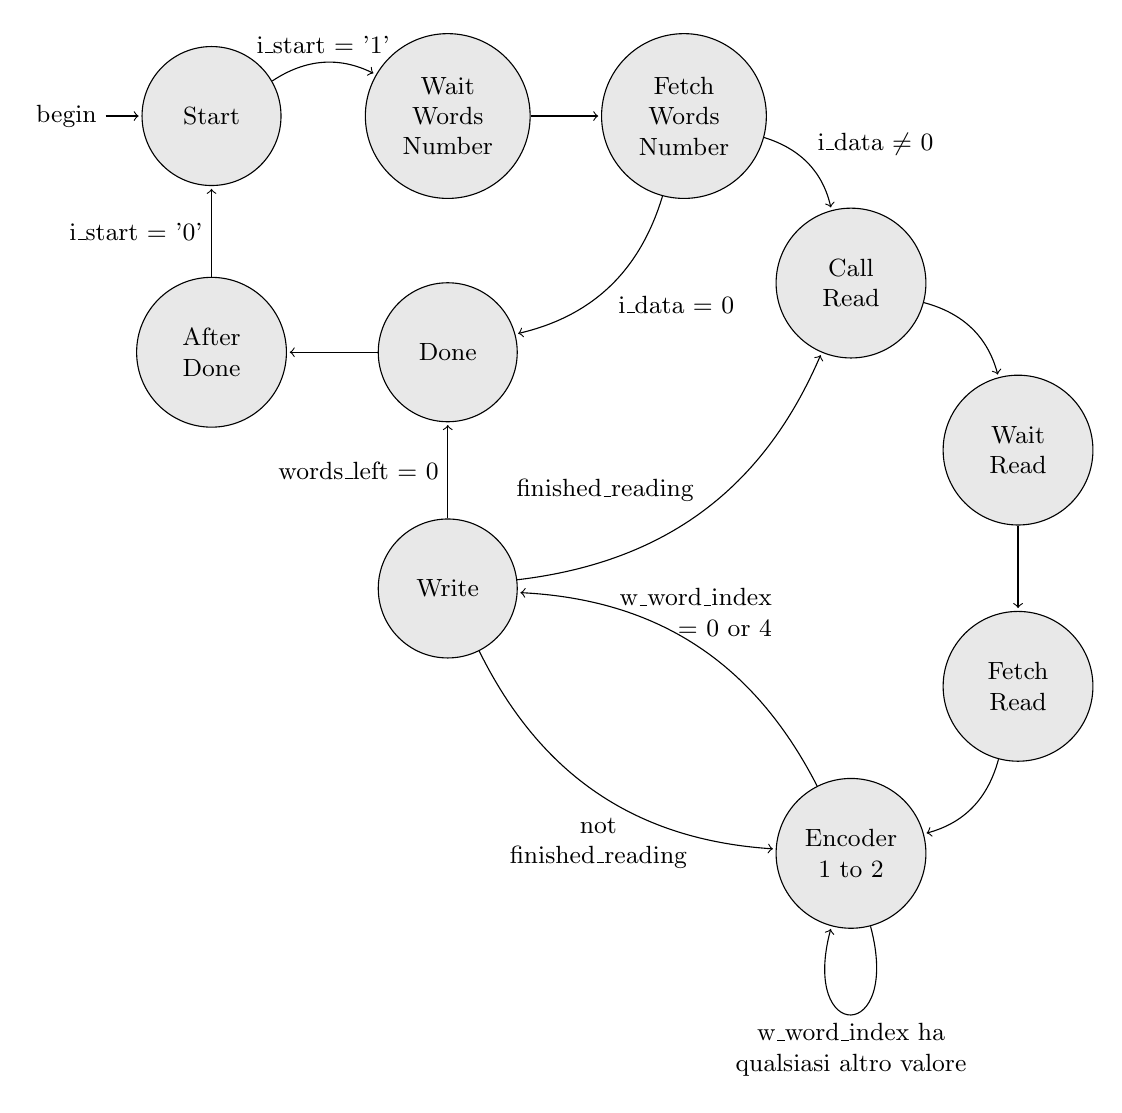
\begin{tikzpicture}[shorten >=1pt,node distance=3cm,node font=\small,on grid,auto,initial text={begin}]
	\tikzstyle{every state}=[fill={rgb:black,1;white,10}]
	
	\node[state,text width=1.5cm,align=center,initial ]  (START)                 {Start};
	\node[state,text width=1.5cm,align=center]                    (WWN) [right of=START]  {Wait\\Words\\Number};
	\node[state,text width=1.5cm,align=center]                    (FWN) [right of=WWN]  {Fetch\\Words\\Number};
	\node[state,text width=1.5cm,align=center]                    (DONE) [below of=WWN]  {Done};
	\node[state,text width=1.5cm,align=center]                    (AD) [left of=DONE]  {After\\Done};
	\node[state,text width=1.5cm,align=center]                    (CR) [below right of=FWN]  {Call\\Read};
	\node[state,text width=1.5cm,align=center]                    (WR) [below right  of=CR]  {Wait\\Read};
	\node[state,text width=1.5cm,align=center]                    (FR) [below of=WR]  {Fetch\\Read};
	\node[state,text width=1.5cm,align=center]                    (WRITE) [below of=DONE]  {Write};
	\node[state,text width=1.5cm,align=center]                    (E12) [below left of=FR]  {Encoder\\1 to 2};
	
	\path[->]
	(START) edge [bend left] node [above] {i\_start = '1'} (WWN)
	(WWN) edge (FWN)
	(FWN) edge [bend left] node {i\_data = 0} (DONE)
	(FWN) edge [bend left] node {i\_data $\ne$ 0} (CR)
	(CR) edge [bend left] (WR)
	(WR) edge (FR)
	(FR) edge [bend left](E12)
	(E12) edge [loop below] node [align=center] {w\_word\_index ha\\qualsiasi altro valore} ()
	(E12) edge [bend right] node [above,align=right] {\\\\w\_word\_index\\= 0 or 4} (WRITE)
	(WRITE) edge [bend right] node [below,align=center] {\\not\\finished\_reading} (E12)
	(WRITE) edge node {words\_left = 0} (DONE)
	(WRITE) edge [bend right] node [align=center] {finished\_reading} (CR)
	(DONE) edge (AD)
	(AD) edge node {i\_start = '0'} (START);
\end{tikzpicture}
\\
\\
\begin{itemize}
	\item \textbf{Start:} Lo stato in cui la macchina è all'inizio dell'esecuzione del programma. In presenza del segnale i\_state = '1' imposta valori iniziali e passa allo stato successivo.
	\item \textbf{Wait Words Number:} Un ciclo di clock dopo che la lettura è stata richiesta riporta a 0 il segnale di lettura.
	\item \textbf{Fetch Word Number:} Dopo la fine della lettura salva il numero di byte in input nella variabile words\_left. Nel caso particolare in cui ci sono 0 byte in ingresso passa direttamente allo stato Done altrimenti incomincia con la lettura del primo byte.
	\item \textbf{Call Read:} Manda segnale di richiesta di lettura e imposta l'indirizzo corretto.
	\item \textbf{Wait Read:} Un ciclo di clock dopo che la lettura è stata richiesta riporta a 0 il segnale di lettura.
	\item \textbf{Fetch Read:} Dopo che la lettura è terminata salva il valore letto in w\_word.
	\item \textbf{Encoder 1 to 2:} In questo stato viene simulato l'automa che effettua la traduzione, lo stato di tale automa è salvato in una variabile separata chiamata internal\_state. Ogni 4 bit tradotti z\_word, ovvero la parola da un byte in uscita, è piena e quindi si passa alla scrittura di tale parola in memoria.
	\item \textbf{Write:} Scrive z\_word in memoria. Dopodiché se rimangono dei bit da leggere in w\_word torna allo stato dell'encoder. Se la parola è finita ma ci sono altre parole in input da leggere torna a Call Reader, se tutte le parole sono state tradotte allora passa a Done.
	\item \textbf{Done:} Manda il segnale o\_done a 1.
	\item \textbf{After Done:} Prima di tornare allo stato Start si assicura che il segnale i\_start che era stato dato all'inizio sia stato riportato a 0. Inotre riporta a 0 il segnale o\_done.
\end{itemize}



\subsection{Macchina a stati finiti?}



%----------------------------------------------------------------------------------------
%	SECTION 3
%----------------------------------------------------------------------------------------

\section{Risultati sperimentali}
\subsection{Sintesi}
Il componente sviluppato è sintetizzabile ed implementabile. 
\begin{figure}[H]
	\centering
	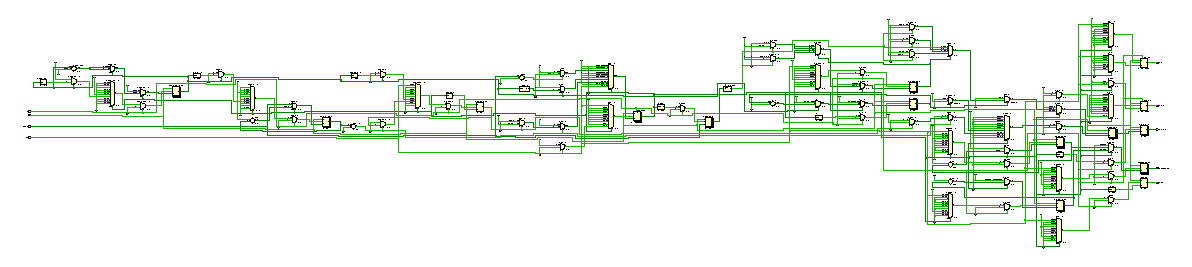
\includegraphics[width=1\textwidth]{Assets/schematic.eps}
	\caption{Schema post-sintesi}
\end{figure}
Nella seguente tabella sono indicati i componenti utilizzati nella sintesi.
\begin{center}
	\begin{tabular}{|c|c|c|c|}
		\hline
		Site Type   & Used & Available & Utilization\% \\
		\hline
		LUT as Logic & 117 & 134600 & 0.09 \\
		\hline
		Register as Flip Flop & 95 & 269200  & 0.04\\
		\hline
		F7 Muxes & 1 & 67300 & <0.01\\
		\hline
	\end{tabular}
\end{center}



\subsection{Simulazioni}
Al fine di verificare il corretto funzionamento del componente sono stati eseguiti diversi test bench in simulazioni Behavioural, Post-synthesis functional e Post-synthesis timing. 
Di seguito sono riportati i test significativi effettuati con relativa spiegazione, tempi ottenuti e grafico d'onda.

\subsubsection{Flussi successivi}
Tramite questo test si verifica la correttezza  nel caso di codifica di più flussi uno dopo l'altro. Nel testbench usato vengono codificati tre flussi (senza reset dopo ogni flusso).
\begin{description}
	\item[Behavioural] 21850 ns
	\item[Post-synthesis functional] 22350100 ps
	\item[Post-synthesis timing] 22353714 ps
\end{description}
\begin{figure}[H]
	\centering
	\includegraphics[width=1\textwidth]{Assets/tb1.png}
	\caption{Post-synthesis functional simulation waveform}
\end{figure}

\subsubsection{Reset asincrono}
Tramite questo test si verifica il corretto funzionamento del reset asincrono.
\begin{description}
	\item[Behavioural] 10650 ns
	\item[Post-synthesis functional] 10750100 ps
	\item[Post-synthesis timing] 10753714 ps
\end{description}
\begin{figure}[!htb]
	\centering
	\includegraphics[width=1\textwidth]{Assets/tb2.png}
	\caption{Post-synthesis functional simulation waveform}
\end{figure}

\subsubsection{Sequenza di lunghezza massima}
\paragraph{}Tramite questo test si verifica il corretto funzionamento nel caso di sequenza di ingresso di lunghezza massima: 255 byte.
\begin{description}
	\item[Behavioural] 332450 ns
	\item[Post-synthesis functional] 332550100 ps
	\item[Post-synthesis timing] 332553714 ps
\end{description}
In questo caso non si riporta grafico della forma d'onda perché non è possibile distinguere i valori che i segnali assumono nella vista "fit".
%\begin{figure}[!htb]
%	\centering
%	\includegraphics[width=1\textwidth]{Assets/tb3.png}
%	\caption{Post-synthesis functional simulation waveform}
%\end{figure}

\subsubsection{Sequenza di lunghezza nulla}
Tramite questo test si verifica il corretto funzionamento nel caso di sequenza di ingresso di lunghezza minima: 0 byte.
\begin{description}
	\item[Behavioural] 950 ns
	\item[Post-synthesis functional] 1050100 ps
	\item[Post-synthesis timing] 1053714 ps
\end{description}
\begin{figure}[H]
	\centering
	\includegraphics[width=1\textwidth]{Assets/tb4.png}
	\caption{Post-synthesis functional simulation waveform}
\end{figure}

\subsubsection{Double processing sulla stessa RAM}
Tramite questo test si verifica il corretto funzionamento nel caso di scrittura sulla stessa RAM.
\begin{description}
	\item[Behavioural] 9250 ns
	\item[Post-synthesis functional] 9550100 ps
	\item[Post-synthesis timing] 9553714 ps
\end{description}
\begin{figure}[H]
	\centering
	\includegraphics[width=1\textwidth]{Assets/tb5.png}
	\caption{Post-synthesis functional simulation waveform}
\end{figure}

\subsubsection{Tests con reset}
Test bench, con reset dopo ogni test, che effettua 1000 test (generati casualmente con uno script Python).
\begin{description}
	\item[Behavioural] 172743250 ns
	\item[Post-synthesis functional] 172943150100 ps
	\item[Post-synthesis timing] 172943153714 ps
\end{description}
In questo caso non si riporta grafico della forma d'onda perché non è possibile distinguere i valori che i segnali assumono nella vista "fit".

\subsubsection{Tests senza reset}
Test bench, senza reset dopo ogni test, che effettua 1000 test (generati casualmente con uno script Python).
\begin{description}
	\item[Behavioural] 172543450 ns
	\item[Post-synthesis functional] 172743350100 ps
	\item[Post-synthesis timing] 172743353714 ps
\end{description}
In questo caso non si riporta grafico della forma d'onda perché non è possibile distinguere i valori che i segnali assumono nella vista "fit".

\subsection{Osservazioni}
Osservazioni su tempo di clock minimo.\\
Osservazioni su come reset non genera ritardi(?).

%----------------------------------------------------------------------------------------
%	SECTION 4
%----------------------------------------------------------------------------------------

\section{Conclusioni}


%----------------------------------------------------------------------------------------

\end{document}